\documentclass[11pt]{report}

\usepackage[polish]{babel}
\usepackage{csquotes}
\DeclareQuoteAlias[]{dutch}{polish}
\usepackage{polski}
\usepackage{geometry}
\usepackage{listings}
\usepackage{xurl}
\usepackage{hyperref}
\usepackage{import}
\usepackage{multirow}
\usepackage{titling}
\usepackage{anyfontsize}
\usepackage[htt]{hyphenat}
\usepackage{xcolor}
\usepackage{graphicx}
\graphicspath{ {./EiWD_zadanie_02_wykresy/} }
\usepackage[
    style=numeric,
    sorting=nty,
    isbn=false,
    backend=biber, %biber EiWD_zadanie_02
]{biblatex}
\addbibresource{EiWD_zadanie_02.bib}

\newcommand{\prowadzacy}{prof. dr hab. inż. Vasyl Martsenyuk}
\newcommand{\temat}{Graficzna wizualizacja danych z użyciem bibliotek \enquote{matplotlib} i \enquote{seaborn}}
\newcommand{\wariant}{1}
\newcommand{\kierunek}{Informatyka}
\newcommand{\stopien}{II}
\newcommand{\tryb}{niestacjonarne}
\newcommand{\semestr}{III}
\newcommand{\grupa}{1}
\newcommand{\nrLab}{2}
\newcommand{\repozytorium}{https://github.com/prybka82-student/eksploracja_i_wizualizacja_danych/tree/zadanie02}

\definecolor{codegreen}{rgb}{0,0.6,0}
\definecolor{codegray}{rgb}{0.5,0.5,0.5}
\definecolor{codepurple}{rgb}{0.58,0,0.82}
\definecolor{backcolour}{rgb}{0.95,0.95,0.92}

\lstdefinestyle{mystyle}{
    backgroundcolor=\color{backcolour},   
    commentstyle=\color{codegreen},
    keywordstyle=\color{magenta},
    numberstyle=\tiny\color{codegray},
    stringstyle=\color{codepurple},
    basicstyle=\ttfamily\footnotesize,
    breakatwhitespace=false,         
    breaklines=true,                 
    captionpos=b,                    
    keepspaces=true,                 
    numbers=left,                    
    numbersep=5pt,                  
    showspaces=false,                
    showstringspaces=false,
    showtabs=false,                  
    tabsize=2
}

\lstset{style=mystyle}

\makeatletter
\renewcommand{\@makechapterhead}[1]{%
\vspace*{0 pt}%
{\setlength{\parindent}{0pt} \raggedright \normalfont
\bfseries\Huge\thechapter.\ #1
\par\nobreak\vspace{40 pt}}}
\makeatother

\newcounter{zadanie}
\newcommand{\zadanie}[1]{
    \refstepcounter{zadanie}
    \filbreak\vspace*{1cm}
    {\noindent\raggedright\Large \textbf{Zadanie~\thezadanie. #1}}
    \vspace{10 pt}\nopagebreak[1]
}

\begin{document}

\title{Eksploracja i wizualizacja danych}
\author{Piotr Rybka}
\date{16.10.2021}

\import{}{EiWD_title_page.tex}

\chapter*{Polecenie}

Na podstawie danych ze zbioru \cite{daneMedyczne} lub danych losowych, wygenerować wykresy analogiczne do przedstawionych na zajęciach.

\zadanie{Wygenerować wykres liniowy}

Załadowanie bibliotek:

\begin{lstlisting}[language=Python]
import matplotlib.pyplot as plt
%matplotlib inline

import numpy as np

import pandas as pd

import os 
\end{lstlisting}

Załadowanie danych:

\begin{lstlisting}[language=Python]
path = r"C:\Users\piotr\Downloads\EiWD_lab_zadanie02\IHME_DAH_DATABASE_1990_2020_Y2021M09D22.CSV"
folder = r"C:\Users\piotr\Documents\Semestr 3\EiWD_zadanie_02_wykresy"

data = pd.read_csv(path, low_memory=False)
\end{lstlisting}

Wygenerowanie wykresu dla co pięćdziesięciotysięcznej wartości:

\begin{lstlisting}[language=Python]
years = data['year'][::50_000]

plt.rcParams["figure.figsize"] = (20,10)
plt.plot(years)
\end{lstlisting}

Uzyskany wykres -- \ref{fig:wykres1}.

\begin{figure}[h]
    \caption{Wykres liniowy (dane rzeczywiste za~\cite{daneMedyczne})}
    \label{fig:wykres1}
    \centering
    \includegraphics[width=.8\textwidth]{output_3_0}
\end{figure}

\zadanie{Wygenerować kilka wykresów obok siebie}

Utworzesie siatki wykresów:

\begin{lstlisting}[language=Python]
fig = plt.figure()
ax0 = fig.add_subplot(2,2,1)
ax1 = fig.add_subplot(2,2,2)
ax2 = fig.add_subplot(2,2,3)
\end{lstlisting}

Wyodrębnienie danych: co dziesięciotysięczna wartość z~kolumny \enquote{elim\_ch} i co tysięczna wartość z~kolumny \enquote{prelim\_est} z pominięciem pierwszy 350 tysięcy:

\begin{lstlisting}[language=Python]
elim_ch = data['elim_ch'][::10_000]
prelim_est = data['prelim_est'][350_000::1_000]
\end{lstlisting}

Wygenerowanie wykresów:

\begin{lstlisting}[language=Python]
ax0.plot(years)
ax1.plot(elim_ch)
ax2.plot(prelim_est)
\end{lstlisting}

Uzyskany wykres -- \ref{fig:wykres2}.

\begin{figure}[h]
    \caption{Kilka wykresów obok siebie (dane rzeczywiste za~\cite{daneMedyczne})}
    \label{fig:wykres2}
    \centering
    \includegraphics[width=.8\textwidth]{output_4_0}
\end{figure}

\zadanie{Wygenerować wykres liniowy i zdefiniować jego formatowanie}

Załadowanie biblioteki generującej losowe dane:

\begin{lstlisting}[language=Python]
from numpy.random import randn
\end{lstlisting}

Wygenerowanie wykresu liniowego zawierającego 30 losowych wartości z przedziału od 0 do 1, przy czym każda kolejna wartość jest dodawana do poprzedniej.
Formatowanie wykresu: zielone punkty połączone linią ciągłą.

\begin{lstlisting}[language=Python]
plt.plot(randn(30).cumsum(), 'go-')
\end{lstlisting}

Uzyskany wykres -- \ref{fig:wykres3}.

\begin{figure}[h]
    \caption{Wykres liniowy z dodanym formatowaniem własnym (dane losowe)}
    \label{fig:wykres3}
    \centering
    \includegraphics[width=.8\textwidth]{output_5_0}
\end{figure}

Inne formatowanie -- wykres w kolorze brązowym, znaczniki w kształcie kółek o wielkości 22 pikseli, linia przerywana o szerokości 1 piksela:

\begin{lstlisting}[language=Python]
plt.plot(years, color='brown', marker='o', markersize=22, linestyle='--', linewidth=1)
\end{lstlisting}

Uzyskany wykres -- \ref{fig:wykres4}.

\begin{figure}[h]
    \caption{Wykres liniowy z dodanym formatowaniem własnym (dane rzeczywiste za~\cite{daneMedyczne})}
    \label{fig:wykres4}
    \centering
    \includegraphics[width=.8\textwidth]{output_6_0}
\end{figure}

\zadanie{Wygenerować wykres liniowy z dodanym wykresem interpolacji liniowej i legendą}

Wygenerowanie losowych danych (30 wartości, suma skumulowana):

\begin{lstlisting}[language=Python]
data = np.random.randn(30).cumsum()
\end{lstlisting}

Wygenerowanie wykresów:

\begin{itemize}
    \item dane właściwe -- wykres czarny podpisany \enquote{Etykieta} wykonany linią przerywaną;
    \item wykres interpolacji liniowej -- wykres czerwony linią ciągłą.
\end{itemize}

\begin{lstlisting}[language=Python]
data = np.random.randn(30).cumsum()
plt.plot(data, 'k--', label='Etykieta')
plt.plot(data, 'r-',  label="steps-post", drawstyle="steps-post")
plt.legend(loc='best')
\end{lstlisting}

Uzyskany wykres -- \ref{fig:wykres5}.

\begin{figure}[h]
    \caption{Wykres liniowy z dodanym wykresem interpolacji liniowej (dane losowe)}
    \label{fig:wykres5}
    \centering
    \includegraphics[width=.8\textwidth]{wykres5}
\end{figure}

\zadanie{Wygenerować wykres liniowy i dodać do niego samodzielnie zdefiniowane etykiety osi}

Wygenerowanie pustego wykresu (zmienna \enquote{ax}) i danych losowych (tysiąc wartości skumulowanych):

\begin{lstlisting}[language=Python]
fig = plt.figure()
ax = fig.add_subplot(1,1,1)
ax.plot(np.random.randn(1000).cumsum())
\end{lstlisting}

Wyznaczenie miejsc na obu osiach, w których mają znaleźć się etykiety:

\begin{lstlisting}[language=Python]
ax.set_xticks([0, 250, 500, 750, 1000])
ax.set_yticks([-50, -25, 0, 25, 50])
\end{lstlisting}

Dodanie etykiet wartości na osi $x$ oraz etykiet obu osi oraz tytułu wykresu przy użyciu słownika (zmienna \enquote{props}):

\begin{lstlisting}[language=Python]
ax.set_xticklabels(['one', 'two', 'three', 'four', 'five'], rotation=90, fontsize='small')

props = {
    'title': 'Tytul',
    'xlabel': 'Kroki',
    'ylabel': 'Wartosci'
}
ax.set(**props)
\end{lstlisting}

Uzyskany wykres -- \ref{fig:wykres6}.

\begin{figure}[h]
    \caption{Wykres liniowy z dodanymi własnymi etykietami (dane losowe)}
    \label{fig:wykres6}
    \centering
    \includegraphics[width=.8\textwidth]{output_8_0}
\end{figure}

\zadanie{Wygenerować kilka wykresów liniowych w różnych kolorach i nałożyć je na siebie}

Uworzenie wykresu zawierającego jeden podwykres:

\begin{lstlisting}[language=Python]
fig = plt.figure(); 
ax = fig.add_subplot(1,1,1)
\end{lstlisting}

Naniesienie losowych wartości i dodanie legenty oraz następującego formatowania:

\begin{itemize}
    \item wykres 1. -- kolor czarny, linia ciągła, etykieta: \enquote{one},
    \item wykres 2. -- kolor czerwony, linia przerywana, etykieta: \enquote{two},
    \item wykres 3. -- kolor zielony, linia kropkowana, etykieta: \enquote{three}.
\end{itemize}

\begin{lstlisting}[language=Python]
ax.plot(randn(1000).cumsum(), 'k', label='one')
ax.plot(randn(1000).cumsum(), 'r--', label='two')
ax.plot(randn(1000).cumsum(), 'g.', label='three')
ax.legend(loc='best')
\end{lstlisting}

Uzyskany wykres -- \ref{fig:wykres7}.

\begin{figure}[h]
    \caption{Kilka wykresów liniowych odróżnionych formatowaniem (dane losowe)}
    \label{fig:wykres7}
    \centering
    \includegraphics[width=.8\textwidth]{output_9_0}
\end{figure}

\zadanie{Zapisać wygenerowany wykres do pliku}

Kod pozwalający na zapisanie wykresu ze wskazaniem rozdzielczości (400 dpi) i szerokości marginesów (wąskie -- \textit{tight}):

\begin{lstlisting}[language=Python]
path = r"C:\Users\piotr\Downloads\wykres01.svg"

plt.savefig(path, dpi=400, bbox_inches='tight')
\end{lstlisting}

\zadanie{Wygenerować wykres liniowy z użyciem indeksu}

Zaimportowanie bibliotek i zdefiniowanie maksymalnego zakresu osi \textit{OX}:

\begin{lstlisting}[language=Python]
import numpy as np
import pandas as pd

xmax = 300_000
\end{lstlisting}

Wygenerowanie wykresu z indeksem zawierającym 50 tysięcy wartości w przedziale od 0 do 1~499~950~000:

\begin{lstlisting}[language=Python]
s = pd.Series(years, index=np.arange(0, xmax*50_000, 50_000))
s.plot(kind='line', logy=False, xticks=[0, xmax/8, xmax/4, xmax/2, xmax], xlim=[0, xmax], grid=True, style='r--')
\end{lstlisting}

Uzyskany wykres -- \ref{fig:wykres8}.

\begin{figure}[h]
    \caption{Wykres liniowy z użyciem indeksu (dane rzeczywiste za~\cite{daneMedyczne})}
    \label{fig:wykres8}
    \centering
    \includegraphics[width=.8\textwidth]{output_11_0}
\end{figure}

\zadanie{Wygenerować kilka wykresów liniowych ułożonych jeden nad drugim}

Wygenerowanie losowych danych (6 serii po 10 losowych wartości każda, serie opatrzone etykietami
\enquote{A}, \enquote{B}, \enquote{C}, \enquote{D}, \enquote{E}, \enquote{F} i 10 indeksami o wartościach 0, 10, 20, 30, 40, 50, 60, 70, 80, 90):

\begin{lstlisting}[language=Python]
df = pd.DataFrame(np.random.randn(10, 6).cumsum(0), columns=['A', 'B', 'C', 'D', 'E', 'F'], index=np.arange(0, 100, 10))
\end{lstlisting}

Wygenerowanie wykresu

\begin{lstlisting}[language=Python]
df.plot(subplots=True, sharex=True, sharey=True, title='Tytul wykresu', sort_columns=True)
\end{lstlisting}

Uzyskany wykres -- \ref{fig:wykres9}.

\begin{figure}[h]
    \caption{Kilka wykresów liniowych o wspólnych osiach \textit{OX} i \textit{OY} (dane losowe)}
    \label{fig:wykres9}
    \centering
    \includegraphics[width=.8\textwidth]{wykres9}
\end{figure}

\zadanie{Wygenerować wykresy słupkowe ułożone poziomo i pionowo}

Wyodrębnienie danych (10 pierwszych danych kolumn \enquote{wb\_location\_id} i \enquote{gbd\_region\_id}):

\begin{lstlisting}[language=Python]
data = pd.DataFrame(num_data[['wb_location_id', 'gbd_region_id']][:10], columns=['gbd_region_id', 'wb_location_id'])
\end{lstlisting}

Wygenerowanie dwóch wykresów (jednego nad drugim -- pierwszy, pionowy w kolorze czarnym, drugi, poziomy -- czerwonym):

\begin{lstlisting}[language=Python]
fig, axes = plt.subplots(2, 1)

data.plot.bar(ax = axes[0], color='k', alpha=0.7)
data.plot.barh(ax = axes[1], color='r', alpha=0.7)
\end{lstlisting}

Uzyskany wykres -- \ref{fig:wykres10}.

\begin{figure}[h]
    \caption{Wykresy słupkowe (dane rzeczywiste za~\cite{daneMedyczne})}
    \label{fig:wykres10}
    \centering
    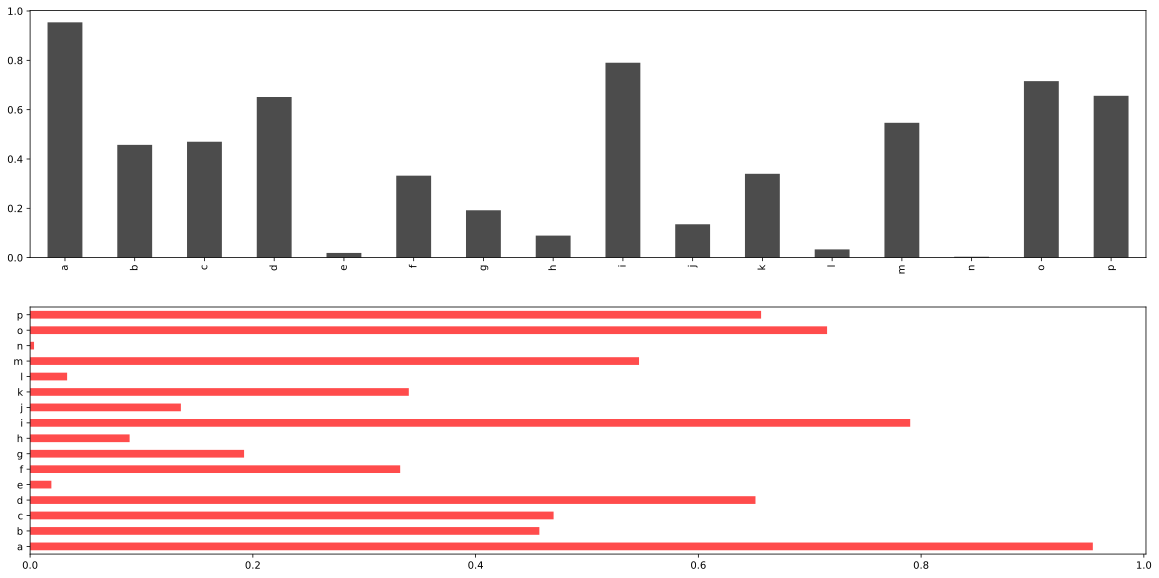
\includegraphics[width=.8\textwidth]{wykres10}
\end{figure}

\zadanie{Wygenerować wykres słupkowy z pogrupowanymi danymi}

Wygenerowanie losowych danych (5 serii po 3 losowe wartości):

\begin{lstlisting}[language=Python]
data = np.random.rand(3, 5)
\end{lstlisting}

Wygenerowanie wykresu słupkowego o nazwie \enquote{Nazwa}. Etykiety serii -- \enquote{a}, \enquote{b}, \enquote{c};
etykiety wartości w każdej serii: \enquote{1}, \enquote{2}, \enquote{3}, \enquote{4}, \enquote{5}:

\begin{lstlisting}[language=Python]
df = pd.DataFrame(data, index=['a', 'b', 'c'], columns=pd.Index(['1', '2', '3', '4', '5'], name='Nazwa'))
df.plot.bar()
\end{lstlisting}

Uzyskany wykres -- \ref{fig:wykres11}.

\begin{figure}[h]
    \caption{Wykresy słupkowe (dane losowe)}
    \label{fig:wykres11}
    \centering
    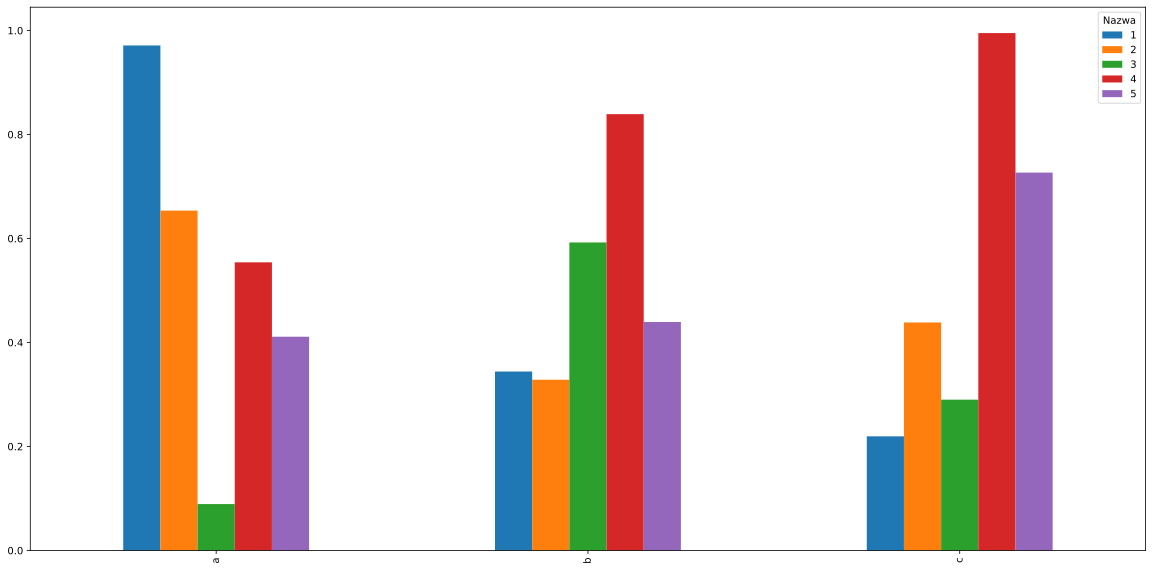
\includegraphics[width=.8\textwidth]{wykres11}
\end{figure}

\zadanie{Wygenerować wykres słupkowy skumulowany}

Wygenerowanie wykresu (dane losowe jak poprzednio):

\begin{lstlisting}[language=Python]
df.plot.bar(stacked=True, alpha=0.8)
\end{lstlisting}

Uzyskany wykres -- \ref{fig:wykres12}.

\begin{figure}[h]
    \caption{Wykres słupkowy skumulowany (dane losowe)}
    \label{fig:wykres12}
    \centering
    \includegraphics[width=.8\textwidth]{wykres12}
\end{figure}

\zadanie{Wygenerować wykres słupkowy przy użyciu biblioteki \textit{seaborn}}

Zaimportowanie biblioteki i wygenerowanie wykresu dla kolumn \enquote{elim\_ch} (oś pionowa) i \enquote{year} (oś pozioma):

\begin{lstlisting}[language=Python]
import seaborn as sns

max = 100_000
per = 1_000
sns.barplot(y=num_data.elim_ch[:max:per], x = num_data.year[:max:per])
\end{lstlisting}

Uzyskany wykres -- \ref{fig:wykres13}.

\begin{figure}[h]
    \caption{Wykres słupkowy wygenerowany przy użyciu biblioteki \texttt{seaborn} z zaznaczeniem 95-proc. przedziłu ufności
        \label{fig:wykres13}
        (dane rzeczywiste za~\cite{daneMedyczne})}
    \centering
    \includegraphics[width=.8\textwidth]{wykres14}
\end{figure}

\zadanie{Wygenerować histogram}

Wygenerowanie histogramu w kolorze zielonym na podstawie danych z~kolumny \enquote{year} (wartości podzielone na 10 grup):

\begin{lstlisting}[language=Python]
num_data['year'].plot.hist(bins=10, color='green')
\end{lstlisting}

Uzyskany wykres -- \ref{fig:wykres14}.

\begin{figure}[h]
    \caption{Histogram (dane rzeczywiste za~\cite{daneMedyczne})}
    \label{fig:wykres14}
    \centering
    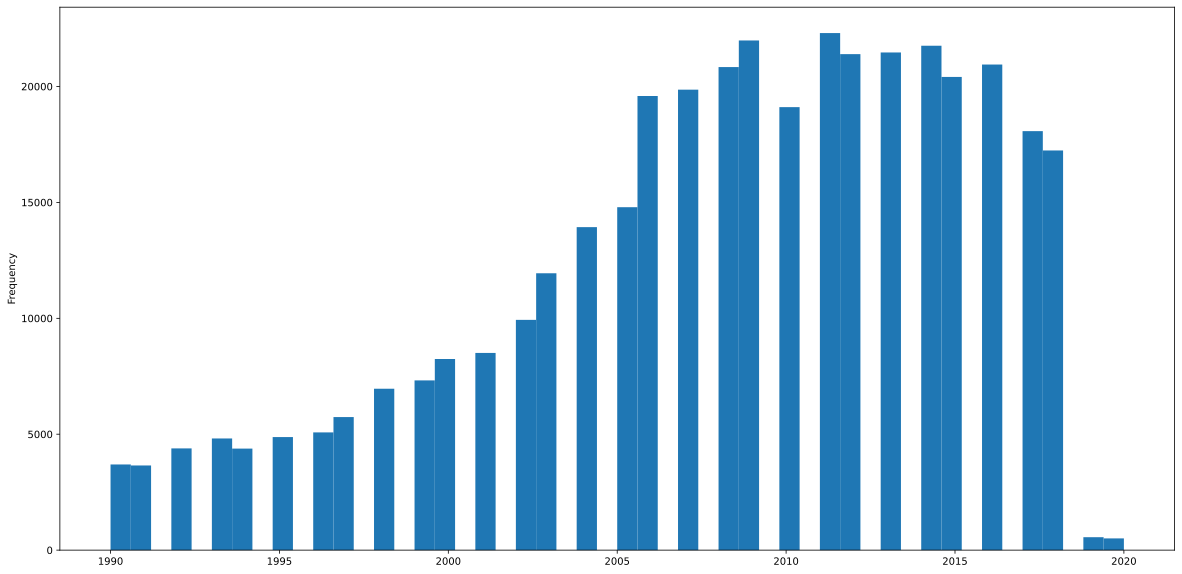
\includegraphics[width=.8\textwidth]{wykres15}
\end{figure}

\zadanie{Wygenerować wykres gęstości prawdopodobieństwa i nałożyć go na histogram}

Wykresy wygenerowanie przy użyciu biblioteki \enquote{pandas} (wykres gęstości w kolorze czerwonym podpisany etykietą \enquote{Density}):

\begin{lstlisting}[language=Python]
# wygenerowanie histogramu
num_data['year'].plot.hist(bins=10, color='green', alpha=0.2)

# wygenerowanie wykresu gestosci
ax = num_data['year'].plot.kde(color='red', linewidth=2.0, secondary_y=True)

# dodanie etykiety do dodatkowego wykresu
ax.set_ylabel("Frequency", fontsize=10)
\end{lstlisting}

Uzyskany wykres -- \ref{fig:wykres15}.

\begin{figure}[h]
    \caption{Wykres gęstości prawdopodobieństwa nałożony na histogram (dane rzeczywiste za~\cite{daneMedyczne})}
    \label{fig:wykres15}
    \centering
    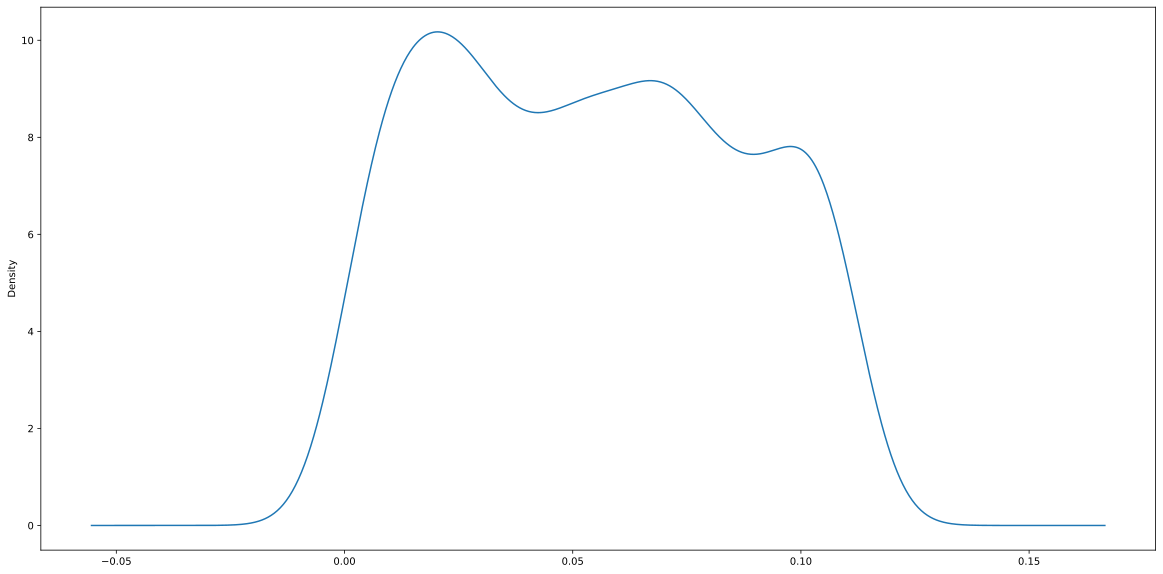
\includegraphics[width=.8\textwidth]{wykres16}
\end{figure}

Taki sam wykres uzyskany przy użyciu biblioteki \enquote{seaborn}:

\begin{lstlisting}[language=Python]
sns.distplot(num_data['year'], bins=10, color='r')
\end{lstlisting}

Uzyskany wykres -- \ref{fig:wykres16}.

\begin{figure}[h]
    \caption{Wykres gęstości prawdopodobieństwa i histogram uzyskany przy użyciu biblioteki \enquote{seaborn} (dane rzeczywiste za~\cite{daneMedyczne})}
    \label{fig:wykres16}
    \centering
    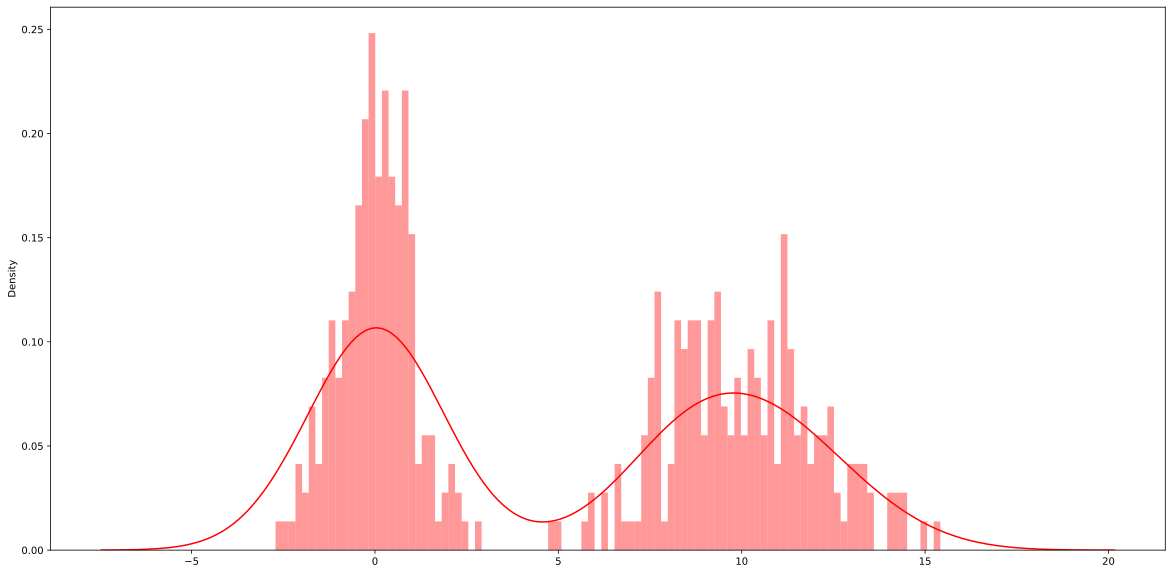
\includegraphics[width=.8\textwidth]{wykres17}
\end{figure}

\zadanie{Wygenerować wykres regresji liniowej}

Wygenerowanie losowych danych:

\begin{lstlisting}[language=Python]
n = 1_000
data = pd.DataFrame({
    'x': np.random.rand(n)*5-2,
    'y': np.random.rand(n)*2+5
})
# roznica logarytmow
data = np.log(data).diff()
\end{lstlisting}

Wygenerowanie wykresu i dodanie tytułu:

\begin{lstlisting}[language=Python]
sns.regplot(x='x', y='y', data=data)
plt.title('Zaleznosc $\log{x}$ od $\log{y}$')
\end{lstlisting}

Uzyskany wykres -- \ref{fig:wykres17}.

\begin{figure}[h]
    \caption{Wykres rozrzutu i regresji liniowej (dane losowe)}
    \label{fig:wykres17}
    \centering
    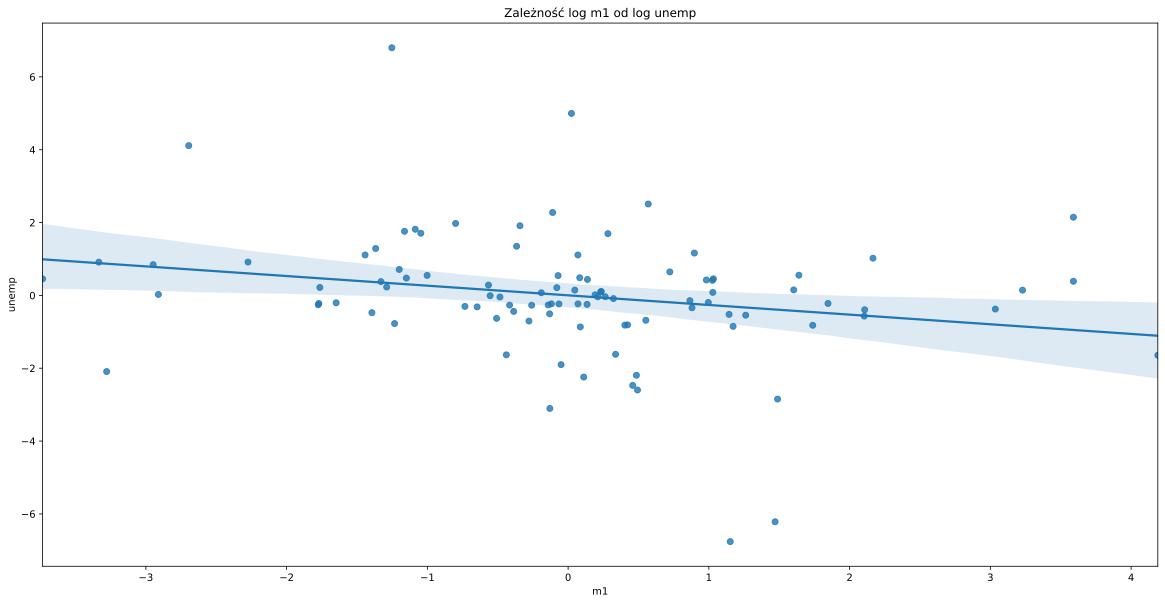
\includegraphics[width=.8\textwidth]{wykres18}
\end{figure}

\zadanie{Wygenerować wszystkie możliwe wykresy rozrzutu oraz wykresy gęstości}

Wygenerowanie wykresu (użyto tych samych danych co w poprzednim zadaniu -- zbiory \enquote{x}, \enquote{y} i \enquote{z}):

\begin{lstlisting}[language=Python]
sns.pairplot(data, diag_kind='kde', plot_kws={'alpha': 0.2})
\end{lstlisting}

Uzyskany wykres -- \ref{fig:wykres18}.

\begin{figure}[h]
    \caption{Wykresy rozrzutu i gęstości prawdopodobieństwa dla różnych zestawień danych (dane losowe)}
    \label{fig:wykres18}
    \centering
    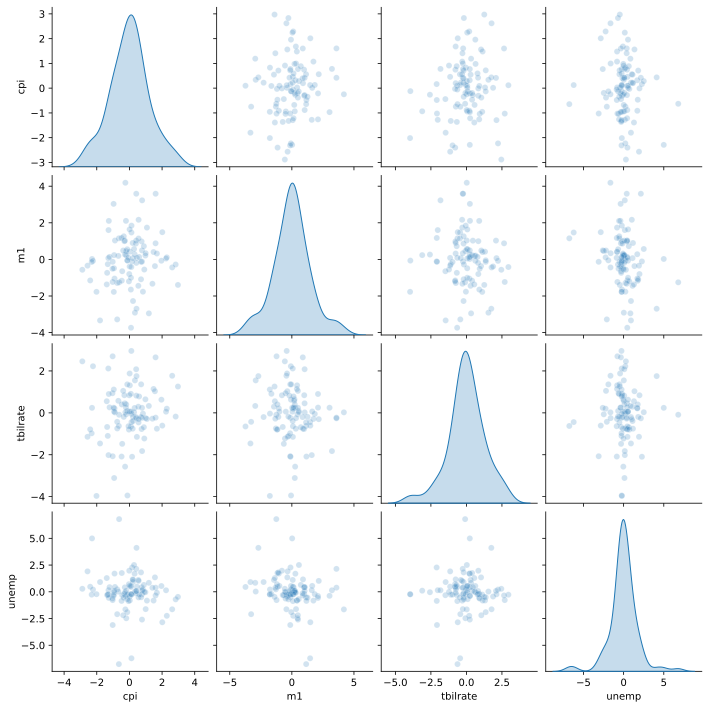
\includegraphics[width=.8\textwidth]{wykres19}
\end{figure}

\zadanie{Wygenerować wykres słupkowy z uwzględnieniem danych kategorycznych}

Pobranie danych i wstępna eksploracja polegająca na ustaleniu, jakie wartości kolumn \enquote{year} i \enquote{source} pojawiają się dla
\enquote{prelim\_est = 0} oraz \enquote{prelim\_est = 1}:

\begin{lstlisting}[language=Python]
path = r"C:\Users\piotr\Downloads\EiWD_lab_zadanie02\IHME_DAH_DATABASE_1990_2020_Y2021M09D22.CSV"

data = pd.read_csv(path, low_memory=False)

print(data.source.drop_duplicates())
print(data[data['prelim_est'] == 1].source.drop_duplicates()) # Australia, Austra, Belgium, Canada, Denmark, Finland, Germany, Greece...
print(data[data['prelim_est'] == 1].year.drop_duplicates()) # 1990, 1991, 2017, 2018, 2019, 2020

print(data.year.drop_duplicates())
print(data[data['prelim_est'] == 0].source.drop_duplicates()) # Australia, Austria, Belgium, Canada, China, Denmark, Finland, France, Germany, Greece...
print(data[data['prelim_est'] == 0].year.drop_duplicates()) # 1990-2020
\end{lstlisting}

Wygenerowanie wykresów słupkowych dla każdej wartości w kolumnie \enquote{prelim\_est}
oraz wybranych państw (kolumna \enquote{source} równa \enquote{Australia}, \enquote{Belgium}, \enquote{Denmark}, \enquote{Finland}, \enquote{Germany})
i lat (kolumna \enquote{year} równa \enquote{2017}, \enquote{2018}, \enquote{2019} i \enquote{2020}):

\begin{lstlisting}[language=Python]
data = data[(data.year.isin([2017, 2018, 2019, 2020]) & data.source.isin(['Austrialia', 'Belgium', 'Denmark', 'Finland', 'Germany']))]

sns.catplot(x='source', y='elim_ch', hue='year', col='prelim_est', kind='bar', data=data)
\end{lstlisting}

Uzyskany wykres -- \ref{fig:wykres19}.

\begin{figure}[h]
    \caption{Wykres słupkowy uwzględniający dane kategoryczne z~kolumny \enquote{prelim\_est} (dane rzeczywiste za~\cite{daneMedyczne})}
    \label{fig:wykres19}
    \centering
    \includegraphics[width=.8\textwidth]{wykres20}
\end{figure}

\zadanie{Wygenerować wykresy słupkowy uwzględniajace dwie kolumny danych kategorycznych}

Dane jak w poprzednim zadaniu. W kodzie generującym wykres znajduje się dodatkowy parametr \enquote{row} wskazujący
na drugą kolumnę kategoryczną \enquote{gbd\_region}, z której wybrano 3 wartości:
\enquote{Asia, South}, \enquote{Asia, East} oraz \enquote{Asia, Central}:

\begin{lstlisting}[language=Python]
    sns.catplot(x='source', y='elim_ch', hue='year', row='gbd_region', col='prelim_est', kind='bar', data=data[data.gbd_region.isin(['Asia, South', 'Asia, East', 'Asia, Central'])])
\end{lstlisting}

Uzyskany wykres -- \ref{fig:wykres20}.

\begin{figure}[h]
    \caption{Wykres słupkowy uwzględniający dane kategoryczne z~kolumn \enquote{gbd\_region} i~\enquote{prelim\_est} (dane rzeczywiste za~\cite{daneMedyczne})}
    \label{fig:wykres20}
    \centering
    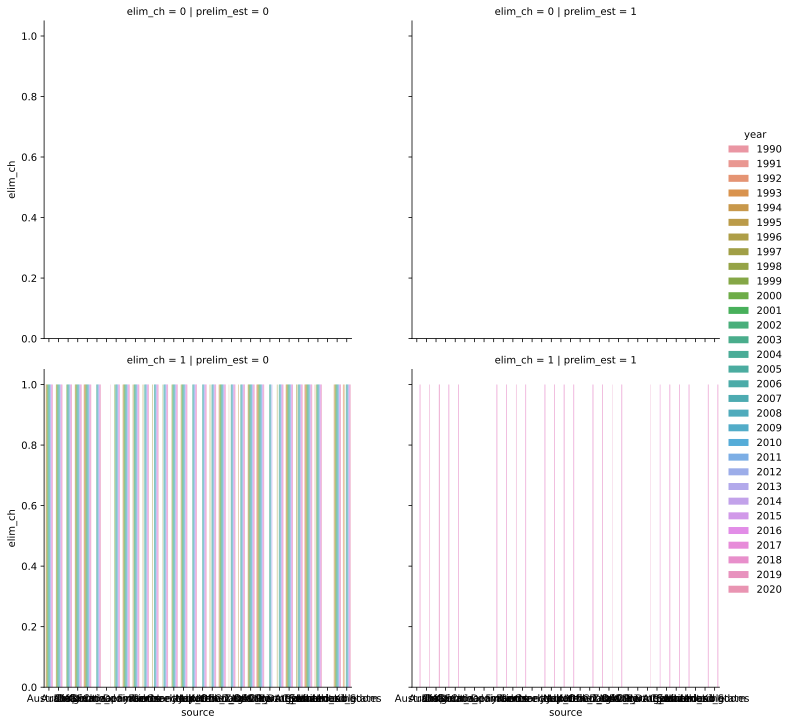
\includegraphics[width=.8\textwidth]{wykres21}
\end{figure}

\zadanie{Wygenerować wykres pudełkowy}

Dodanie kolumny \enquote{swap\_hss\_total\_dah\_20\_num} zawierającej zero lub
wartość logarytmu przy podstawie 10 z wartości w kolumnie \enquote{swap\_hss\_total\_dah\_20} przekonwertowanej do liczby całkowitej
i powiększonej o 1:

\begin{lstlisting}[language=Python]
import math

data['swap_hss_total_dah_20_num'] = data.swap_hss_total_dah_20.apply(lambda x: 0 if x=='-' else math.log(abs(int(x)+1),10))
\end{lstlisting}

Wygenerowanie wykresu pudełkowego dla wartości w kolumnie \enquote{swap\_hss\_total\_dah\_20\_num} pogrupowanych względem wartości
w kolumnie \enquote{source}:

\begin{lstlisting}[language=Python]
sns.catplot(x='source', y='swap_hss_total_dah_20_num', kind='box', data=data)
\end{lstlisting}

Uzyskany wykres -- \ref{fig:wykres21}.

\begin{figure}[h]
    \caption{Wykres pudełkowy wartości w kolumnie \enquote{swap\_hss\_total\_dah\_20\_num} pogrupowanych względem wartości w kolumnie \enquote{source} (dane rzeczywiste za~\cite{daneMedyczne})}
    \label{fig:wykres21}
    \centering
    \includegraphics[width=.8\textwidth]{wykres22}
\end{figure}

\chapter*{Wnioski}

Biblioteki \enquote{matplotlib} i \enquote{seaborn} pozwalają generować następujące rodzaje wykresów:

\begin{itemize}
    \item wykresy liniowe:

          \begin{lstlisting}[language=Python]
import matplotlib.pyplot as plt

plt.plot(ramka_danych)
\end{lstlisting}

    \item wykresy liniowe: \texttt{ramka\_danych.plot(kind='line', 'k--')},
    \item wykresy słupkowe pionowe: \texttt{ramka\_danych.plot.bar(color = 'k')},
    \item wykresy słupkowe poziome: \texttt{ramka\_danych.plot.barh(color = 'r')},
    \item wykresy słupkowe skumulowane: \texttt{ramka\_danych.plot.bar(stacked=True)},
    \item wykresy słupkowe z przedziałami ufności (biblioteka \enquote{seaborn}): \\ \texttt{seaborn.barplot(y=ramka.daneA, x=ramka.daneB)},
    \item wykresy słupkowe z danymi kategorycznymi:

          \begin{lstlisting}[language=Python]
# jedna kategoria -- kolumnaD
seaborn.catplot(x='kolumnaA', y='kolumnaB', kind='bar',
    hue='kolumnaC_podkategorie_odrozniane_kolorem', 
    col='kolumnaD_podkategorie_na_podwykresach', 
    data=ramka_danych)

# dwie kategorie -- kolumnaD i kolumnaE
seaborn.catplot(x='kolumnaA', y='kolumnaB', kind='bar',
    hue='kolumnaC',
    col='kolumnaD',
    row='kolumnaE',
    data=ramka_danych)
\end{lstlisting}

    \item histogramy: \texttt{ramka\_danych.plot.hist(bins=10)},
    \item wykresy gęstości prawdopodobieństwa: \texttt{ramka\_danych.plot.kde(color = 'g')},
    \item histogram z nałożonym wykresem gęstości prawdopodobieństwa:

          \begin{lstlisting}[language=Python]
# biblioteka pandas
ramka_danych.plot.hist(bins=10)
podwykres = ramka_danych.plot.kde(secondary_y=True)
podwykres = set_ylabel("Etykieta wykresu gestosci", fontsize=10)

# biblioteka seaborn
seaborn.distplot(ramka_danych, bins=10)
\end{lstlisting}

    \item wykresy regresji liniowej: \texttt{seaborn.regplot(x='kolumna\_a\_ramki', y='kolumna\_b\_ramki', data=ramka\_danych)},
    \item wykresy rozrzutu: \texttt{seaborn.pairplot(ramka\_danych, diag=kind='kde')},

    \item wykresy pudełkowe: \texttt{seaborn.catplot(kind='box', x='kolumnaA', y='kolumnaB', data=ramka\_danych)}

\end{itemize}

Parametry pozwalające formatować wykres:

\begin{itemize}
    \item biblioteka  \texttt{matplotlib.pyplot} funkcja \texttt{plot()}:
          \begin{itemize}
              \item kolor wykresu: \texttt{plt.plot(color='brown')}, \texttt{plt.plot(color='k')},
              \item przeźroczystość wykresu: \texttt{plt.plot(alpha=0.1)}
              \item kształt punktorów: \texttt{plt.plot(marker='o')}, \texttt{plt.plot(marker='.')},
              \item wielkość punktorów: \texttt{plt.plot(markersize=22)},
              \item rodzaj linii: \texttt{plt.plot(linestyle='-')}, \texttt{plt.plot(linestyle='.')},\\ \texttt{plt.plot(linestyle='--')},
              \item szerokość linii: \texttt{plt.plot(linewidth=1)},
              \item kolor i rodzaj linii jednocześnie: \texttt{plt.plot(dane, 'k--')},
              \item etykieta wykresu: \texttt{plt.plot(label='Etykieta')},
              \item położenie legendy (etykiet): \texttt{plt.legend(loc='best'), \texttt{plt.legend(loc='upper left')}, \texttt{plt.legend(loc='center right')}},
              \item położenie etykiet na osiach: \texttt{plt.set\_xticks([0, 100, 200])}, \texttt{plt.set\_yticks([0, 100, 200])},
              \item etykiety osi: \texttt{plt.set\_xticklabels(['a', 'b', 'c'], rotation=90, fontsize='small')},
              \item tytuł wykresu: \texttt{plt.plot(title='Tytul')},
              \item dodanie etykiet przy użyciu słownika:

                    \begin{lstlisting}[language=Python]
            etykiety = {
                'title': 'Tytul',
                'xlabel': 'Etykiety osi OX',
                'ylabel': 'Etykiety osi OY'
            }
            
            plt.set(**etykiety)
        \end{lstlisting}

              \item wartości w skali logarytmicznej: \texttt{ramka\_danych.plot(logy=True)},
              \item siatka: \texttt{ramka\_danych.plot(grid=True)},
              \item zakres osi: \texttt{ramka\_danych.plot(xlim=[0, 100])};

          \end{itemize}

\end{itemize}

Generowanie kilku wykresów na jednym rysunku:

\begin{lstlisting}[language=Python]
import matplotlib.pyplot as plt

# funkcja figure i kilka ramek danych:
ilustracja = plt.figure()
wykres1 = ilustracja.add_subplot(2,2,1)
wykres2 = ilustracja.add_subplot(2,2,2)
wykres3 = ilustracja.add_subplot(2,2,3)

wykres1.plot(ramka_danych1)
wykres2.plot(ramka_danych2)
wykres3.plot(ramka_danych3)

# funkcja plot z parametrem subplots i jedna ramka danych, wspolna os OX:
ramka_danych.plot(subplots=True, sharex=True, sharey=False, title='Tytul', sort_columns=True)
\end{lstlisting}

Zapis do pliku:

\begin{lstlisting}[language=Python]
    plt.savefig(sciezka_pliku, dpi=300, bbox_inches='tight')
\end{lstlisting}

%\cleardoublepage

\printbibliography[heading=subbibliography,title={Strony internetowe},keyword=www]

\end{document}